\section{Methodology}
The simulation is conducted through Simulink, as depicted in Fig~\ref{fig:heat_system_diagram} the heating or control temperature system. This system comprises four primary components: the heating system, the $P_{0}$ computation, the $x_{0}$ calculation, and the least-squares filter implemented as a Matlab function.

\begin{figure}[H]
\centering
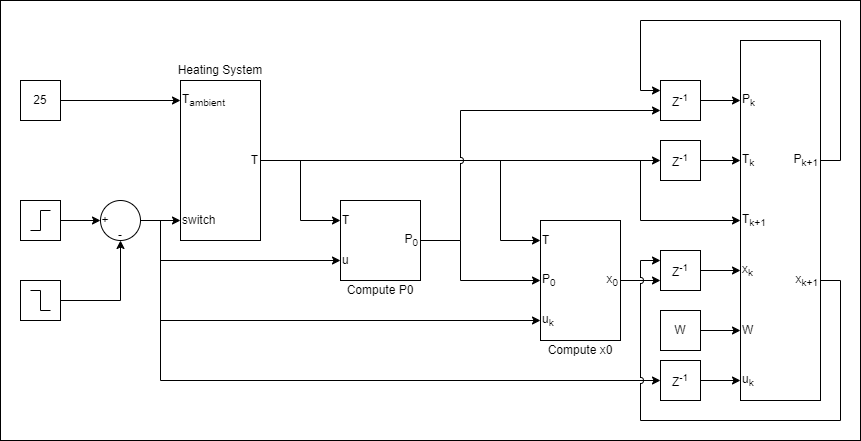
\includegraphics[width=1\linewidth]{figures/heat_system_diagram.png}
\caption{Diagram representing the complete system to be simulated}
~\label{fig:heat_system_diagram}
\end{figure}

The heating system is responsible for replicating the temperature variation, using an ambient temperature of 25$^{\circ}$C as a reference. There are two tested scenarios. In the first one, the simulation begins with a transition from 0$^{\circ}$C to 25$^{\circ}$C. Subsequently, the heating system activates, initiating a temperature alteration over a 150-second interval. Following this, the system deactivates and the simulation runs for an additional 150-second period. In the second scenario, there is a square input function that has a period of 20s and an amplitude of 100. The simulation runs for 400 seconds in order to have more data and see how the system improves over time. \\

The component that computes $P_{0}$ uses the Eq~\ref{eq:lse_recursion_P0}. The following Matlab code shows its implementation:

\lstinputlisting[language=Octave]{codes/compute_p0.m}

In the other hand, Eq~\ref{eq:lse_recursion_x0} is used to compute the value of $x_{0}$ and the implemented code is shown:

\lstinputlisting[language=Octave]{codes/compute_x0.m}

Finally, the least-squares estimation using the covariance recursion form based on Eq~\ref{eq:lse_recursion} is implemented as shown below:

\lstinputlisting[language=Octave]{codes/compute_pk1.m}

For the simulation, the following parameters are used:

\begin{itemize}
    \item $\tau$: the time constant of the system is set to 20s.

    \item $K_{p}$: the gain of the system is set to 0.5.

    \item $\sigma$: the standard deviation of the Gaussian white noise is set to 0.008.

    \item $\alpha$: is set to $10^{3}$

    \item $\beta$: is vector set to $\left[ 0.01 ~ 0.01 \right]$.

    \item $\Delta t$: the sampling time is set to 0.1 seconds.
\end{itemize}

and the code used is shown, as well as the computation of the parameters $a$, $b$, and $W$:

\lstinputlisting[language=Octave]{codes/constants.m}

where:

\begin{equation}
    a = \frac{-1}{\tau} = \frac{-1}{20} = -0.05
\end{equation}

\begin{equation}
    b = \frac{K_{p}}{\tau} = \frac{0.5}{20} = 0.025
\end{equation}

\begin{equation}
    W = \frac{1}{\sigma^{2}} = \frac{1}{0.08^{2}} = 156.25
\end{equation}

The system predicts the parameters $\phi$ and $\Gamma$ which can be computed using the Eq~\ref{eq:phi} and~\ref{eq:gamma}:

\begin{equation}
    \phi(k) = e^{a \cdot \Delta t} = e^{-0.05 \cdot 0.1} = 0.9950
\end{equation}

\begin{equation}
    \Gamma(k) = \frac{0.025}{-0.05} \left( e^{-0.05 \cdot 0.1} - 1\right) = 0.002494
\end{equation}

